\documentclass{beamer}
%\mode<presentation>
\usepackage[utf8]{inputenc}
%\usepackage[english]{babel}
\usepackage[magyar]{babel}
\usetheme{CambridgeUS}
\usecolortheme{dolphin}
\usepackage{amsmath,amssymb,amsfonts, bm}
\usepackage{mathpazo}
\usepackage{graphicx,tabularx,epsfig}
\usepackage[compatibility=false]{caption}
\usepackage{subcaption}
\usepackage{rotating}
\DeclareGraphicsExtensions{.pdf,.png,.jpg,.svg}



\setbeamertemplate{background}{\tikz[overlay,remember picture]\node[opacity=0.07]at (current page.center){\includegraphics[width=\paperwidth]{pic/bkg}};}
\usepackage{tikz}

\setbeamertemplate{itemize items}[square]
\setbeamertemplate{enumerate items}[square]

\definecolor{Red}{RGB}{190,0,0}
\definecolor{Blue}{RGB}{0,0,190}




\title[Numerical hydrodynamics]{Time evolution of the spatial anisotropies in heavy ion collisions}
\author[Attila Bagoly]{\underline{Attila Bagoly}, Máté Csanád \vspace{0.5cm}}
\institute[ELTE]{\large{Eötvös Loránd University} \\ \normalsize{Department of Atomic physics}}

\date[\today]{16. Zimányi WINTER SCHOOL ON HEAVY ION PHYSICS \\ \today}
\begin{document}

\begin{frame}
  \titlepage
\end{frame}


\section{Introduction}

\begin{frame}
\frametitle{Motivation}

How fluidity of sQGP  determine:
\vspace{10pt}
	\begin{itemize}
		  \setlength{\itemsep}{8pt}
		\item<1-> how simple effects influence time evolution of asymmetries
		\item<1-> effects which can't be discussed analytically 
	\end{itemize}
\vspace{20pt}
$\Longrightarrow$ Numerical hydrodynamics: realistic models, but effects get mixed
\vspace{20pt}


$\Longrightarrow$ Initial condition: close to exact solution, but more realistic
\vspace{20pt}


\textcolor{red}{\underline{Published}:} Int. J. Mod. Phys. A 31, 1645016 (2016)

 %\textcolor{blue}{DOI: 10.1142/S0217751X16450160}

\end{frame}

\begin{frame}
\frametitle{Table of contents}
\begin{enumerate}
  \setlength{\itemsep}{14pt}
\item<1-> Equations of hydrodynamics
\item<1-> Numerical method
\item<1-> Code testing
\item<1-> Initial conditions
\item<1-> Reaction planes
\item<1-> Nonrelativistic results
\item<1-> Relativistic results
\item<1-> Hadronization

\end{enumerate}

\end{frame}

\section{Equations of hydrodynamics}
\begin{frame}
\frametitle{Equations of hydrodynamics}
\begin{itemize}
\item<1-> Nonrelativistic :
\begin{itemize}
\item<1-> Barion number conservation:\quad \begin{large}$\dfrac{\partial \rho}{\partial t} + \bm{\nabla}\rho\bm{v}=0$\end{large}
\item<1-> Impulse conservation:\quad \begin{center}\begin{large}$\rho\Big(\dfrac{\partial \bm{v}}{\partial t}+(\bm{v\nabla})\bm{v}\Big)=-\bm{\nabla}p +\mu\Delta\bm{v}+\Big(\zeta+\dfrac{\mu}{3}\Big)\bm{\nabla}(\bm{\nabla v})+\bm{f}$\end{large}\end{center}
\item<1-> Energy conservation: \quad\begin{large}$\dfrac{\partial \varepsilon}{\partial t}+\bm{\nabla}\varepsilon\bm{v}=-p\bm{\nabla v}+\bm{\nabla(\sigma v)}$\end{large}
\item<1-> $\rho$ barion number density, $\bm{v}$ velocity field, $\varepsilon$ energy density, $p$ pressure distribution
\end{itemize}

\item<1-> Relativistic hydrodynamics:
\begin{Large}
\begin{center}$T^{\mu\nu}=\big(\varepsilon+p\big)u^\mu u^\nu-pg^{\mu\nu},\quad \partial_\mu T^{\mu\nu}=0$\end{center}
\end{Large}
\begin{itemize}
\item<1-> $T^{\mu\nu}$ energy-impulse tensor, $u^\mu$ four-velocity, $g^{\mu\nu}$ metric tensor
\end{itemize}

\item<1-> Equation of state:\quad \begin{large}$\varepsilon=\kappa(T)p\quad$\end{large} ($\kappa=1/c_s^2$, $\kappa=3/2$ ideal gas)

\item<1-> Advection form: $\partial_t Q(\rho, \varepsilon, \bm{v})+\partial_x F(Q)=0$ $\quad$ ($F$ flux)

\end{itemize}
\end{frame}


%\begin{frame}
%\frametitle{Multipole solution}
%  \begin{minipage}{0.39\textwidth}
%    \includegraphics[scale=0.16]{pic/a1}

%    \includegraphics[scale=0.2]{pic/a2}
%  \end{minipage}
%  \begin{minipage}{0.60\textwidth}
%  \begin{itemize}
%\item New exact solution of relativistic hydrodynamics by Máté Csanád and András Szabó, published Phys.Rev. C90 (2014) 054911
%\item The solution in cylindrical coordinates:
%$u^\mu=\frac{x^\mu}{\tau}$, $n=n_f\big(\frac{\tau_f}{\tau}\big)^3\nu(s)$, $p=p_f\big(\frac{\tau_f}{\tau}\big)^{3+3/\kappa}$
%\item Where $\tau$ is the coordinate-proper time, $\tau_f$ is the freeze-out proper time
%\item The s scale variable with any asymmetries 
%$s=\frac{r^N}{R^N}\Big(1+\epsilon_{N}\cos N\phi\Big)+\frac{z^N}{R^N}$
%\item That's a solution if $R=u_tt$
%\end{itemize}
%  \end{minipage}
%\end{frame}

\section{Numerical scheme}
\begin{frame}
\frametitle{Numerical scheme}
\begin{itemize}
  \setlength{\itemsep}{5pt}

\item<1-> Mid rapidity: distributions have maximum:  $2+1$ dimension
\item<1-> Numerical solution: discretization $\leftarrow$ finite volume method
%\item<3-> Véges térfogat módszer: mennyiségek átlaga rácspont körül
\item<1-> Problem: we need fluxes between grid points $\rightarrow$ approximations
\item<1-> Instability: perturbation, vanish in grid points $\rightarrow$ CFL condition
\item<1-> 2 spatial dimension complicated $\rightarrow$ operator splitting
\item<1-> Viscosity: ideal substep + viscous substep (operator splitting)
\end{itemize}
\begin{center}
\includegraphics<1->[scale=0.19]{pic/f1}
\end{center}
\end{frame}

\subsection{MUSTA}
\begin{frame}
\frametitle{MUSTA method}
\begin{itemize}
\item<1-> $\mathrm{n^{th}}$ time step: $Q^{(0)}_i\equiv Q^n_i$,  $Q^{(0)}_{i+1}\equiv Q^{n}_{i+1}$
\item<1-> $\ell^\mathrm{th}$ predicted values: $Q^{(\ell)}_{i}$, $F^{(\ell)}_{i}\equiv F\big(Q^{(\ell)}_{i}\big)$
\item<1-> Intermediate value and flux:
\begin{equation*}
Q^{(\ell)}_{i+\frac{1}{2}}=\frac{1}{2}\Big[Q^{(\ell)}_i+Q^{(\ell)}_{i+1}\Big]-\frac{1}{2}\frac{\Delta t}{\Delta x}\Big[F^{(\ell)}_{i+1}-F^{(\ell)}_i\Big], \quad F_M^{(\ell)} \equiv F\big(Q^{(\ell)}_{i+\frac{1}{2}}\big)
\end{equation*}

\item<1-> Corrected inner flux:
\begin{equation*}
F^{(\ell)}_{i+\frac{1}{2}}=\frac{1}{4}\Big[F^{(\ell)}_{i+1}+2F^{(\ell)}_M+F^{(\ell)}_{i}-\frac{\Delta x}{\Delta t}\Big(Q^{(\ell)}_{i+1}-Q^{(\ell)}_i\Big)\Big]
\end{equation*}
\item<1-> Next prediction to $Q$ values to better approximation of flux:
\begin{equation*}
Q_i^{(\ell+1)}=Q^{(\ell)}_i-\frac{\Delta t}{\Delta x}\Big[F^{(\ell)}_{i+\frac{1}{2}}-F^{(\ell)}_i\Big]
\end{equation*}
%\begin{equation*}
%Q_{i+1}^{(l+1)}=Q^{(l)}_{i+1}-\frac{\Delta t}{\Delta x}\Big[F^{(l)}_{i+1}-F^{(l)}_{i+\frac{1}{2}}\Big]
%\end{equation*}
\item<1-> $\mathit\mathbf{{k}}$ step $\rightarrow$ $F_{i+\frac{1}{2}}=F_{i+\frac{1}{2}}^{(\mathit\mathbf{{k}})}$ $\Longrightarrow\; Q^{n+1}_i=Q^{n}_i-\frac{\Delta t}{\Delta x}(F_{i+\frac{1}{2}}-F_{i-\frac{1}{2}})$
\item<1-> Method published by E. F. Toro et al, 2006, J. Comp. Phys
\end{itemize}
\end{frame}

\subsection{Code testing}
\begin{frame}
\frametitle{Code testing}
\begin{itemize}
  \setlength{\itemsep}{5pt}
\item<1-> Exact solutions (Csörgő et al, PhysRevC67)
\item<1-> Relative difference between numerical and exact solution:
\begin{equation*}
\int{|\rho_{\rm{analytical}}(t,\underline{x})-\rho_{\rm{numerical}}(t,\underline{x})|d^2x}\bigg/\int{\rho_{\rm{analytical}}(t,\underline{x})}d^2x
\end{equation*}
\item<1-> Relativistic code: tested with Karpenko's hydro code
\end{itemize}
\begin{center}
%\visible<1->{$X=Y$ \qquad\qquad\qquad\qquad\qquad\qquad\qquad $X\neq Y$}
\begin{figure}[H]
	\centering
    \begin{subfigure}[b]{0.49\textwidth}
    		\includegraphics<1->[width=\textwidth]{pic/sym}
	\end{subfigure}
	\begin{subfigure}[b]{0.49\textwidth}
        	\includegraphics<1->[width=\textwidth]{pic/asym}
	\end{subfigure}
\end{figure}
\end{center}
\end{frame}


\subsection{Initial condition}
\begin{frame}
\frametitle{Initial condition}
\begin{itemize}
  \setlength{\itemsep}{6pt}
\item<1-> Variables: space dependency only in scale variable, asymmetry in this variable
\item<1-> Number density, pressure \large{$\propto \exp{(-s)}$}
\item<1-> Scale variable: 
\begin{equation*}
s=\frac{r^2}{R^2}\Big(1+\textcolor{Red}{\epsilon_2}\cos(2\phi)+\textcolor{Red}{\epsilon_3}\cos(3\phi)+\textcolor{Red}{\epsilon_4}\cos(4\phi)\Big)
\end{equation*}
\begin{center}
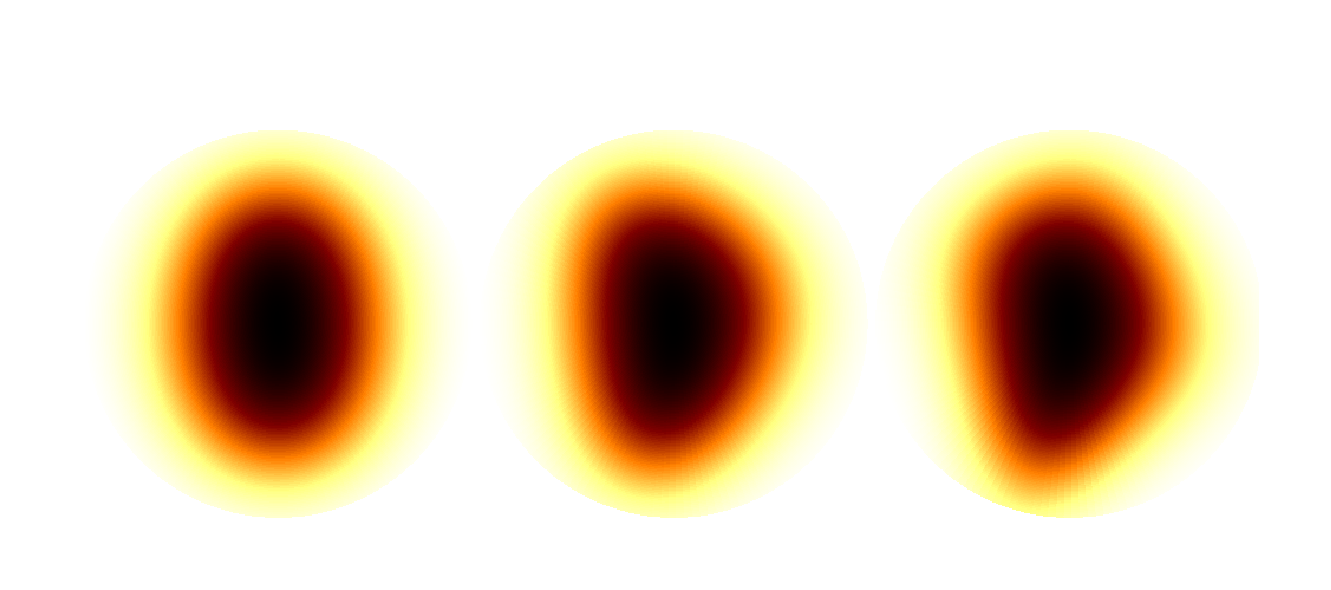
\includegraphics[scale=0.15]{pic/ic}
\end{center}
\item<1-> Velocity: Hubble-velocity field or $0$
\item<1-> Effect of pressure gradient: \large{$p \propto \exp{(-\rm{c_p}\cdot s)}$}
\item<1-> Constant pressure, multipole exact solution: Csanád és Szabó, \\Phys.Rev. C90 (2014) 054911
\end{itemize}
\end{frame}

\begin{frame}
\frametitle{More realistic initial condition}
\begin{itemize}
  \setlength{\itemsep}{12pt}
\item<1-> Gaussian decay $\rightarrow$ values in full space ($\Omega$)
\item<1-> Better model: Gaussian decay in $\mathcal{A}\subset \Omega$, $0$ in $\Omega \setminus \mathcal{A}$
\item<1-> Problem: numerical instability at $\partial \mathcal{A}$ (non existing derivates)
\item<1-> Idea: $exp(-s)\rightarrow$ smooth function, example:
\begin{equation*}
{\displaystyle f(x)={\begin{cases}e^{-{\frac {1}{1-x^{2}}}}&{\text{ if }}|x|<1,\\0&{\text{ otherwise }}\end{cases}}}
\end{equation*}
\item<1-> Member of $C^{\infty}$ but not good for analyzing asymmetries
\item<1-> Other idea: keep $\exp{-s}$ distribution for $\mathcal{A}$, $0$ for $\Omega\setminus\mathcal{A}$

\item<1-> But: convolved with $f(x)$ $\rightarrow$ smooth function, derivates will be OK at boundary

\end{itemize}
\end{frame}


\subsection{Description of asymmetries}
\begin{frame}
\frametitle{Description of asymmetries}
\begin{itemize}
  \setlength{\itemsep}{14pt}
\item<1-> Scale variable: $s=\frac{r^2}{R^2}\big(1+\textcolor{Red}{\epsilon_2}\cos(2\phi)+\textcolor{Red}{\epsilon_3}\cos(3\phi)+\textcolor{Red}{\epsilon_4}\cos(4\phi)\big)$
\item<1-> Definition of asymmetry parameters: $\textcolor{Blue}{\varepsilon_n}=\langle \cos(n\phi)\rangle_{\rho/\bm{v}/p}$
\item<1-> $\textcolor{Blue}{\varepsilon_n}$ (newly introduced)  $\neq$ $\textcolor{Red}{\epsilon_m}$  (in scale variable)
\item<1-> Initially ($t=0$) connection between $\textcolor{Blue}{\varepsilon_n}$ and $\textcolor{Red}{\epsilon_m}$ can be derived (Taylor expansion):
\vspace{10pt}
\begin{itemize}
 \setlength{\itemsep}{8pt}
\item<1-> $\textcolor{Blue}{\varepsilon_1}=0+\textcolor{Red}{\epsilon_3}(\textcolor{Red}{\epsilon_2}+\textcolor{Red}{\epsilon_4})+\mathcal{O}(\textcolor{Red}{\epsilon^4})$
\item<1-> $\textcolor{Blue}{\varepsilon_2}=-\textcolor{Red}{\epsilon_2}+\textcolor{Red}{\epsilon_2}\textcolor{Red}{\epsilon_4}+\textcolor{Red}{\epsilon_2}\sum_{n} \textcolor{Red}{\epsilon_n^2}+\mathcal{O}(\textcolor{Red}{\epsilon^4})$
\item<1-> $\textcolor{Blue}{\varepsilon_3}=-\textcolor{Red}{\epsilon_3}+\textcolor{Red}{\epsilon_3}\sum_n \textcolor{Red}{\epsilon_n^2}+\mathcal{O}(\textcolor{Red}{\epsilon^4})$
\item<1-> $\textcolor{Blue}{\varepsilon_4}=-\textcolor{Red}{\epsilon_4}+\frac{1}{2}\textcolor{Red}{\epsilon_2^2}-\textcolor{Red}{\epsilon_4}\sum_n\textcolor{Red}{\epsilon_n^2}+\mathcal{O}(\textcolor{Red}{\epsilon^4})$
\end{itemize}
\end{itemize}

\end{frame}

\begin{frame}
\frametitle{Generalize the asymmetry parameters}
\begin{itemize}
  \setlength{\itemsep}{18pt}
\item<1-> $\textcolor{Blue}{\varepsilon_i}$ evolve in time, it freezes out with phase transition $\rightarrow$ $v_n$ parameters
\item<1-> Measuring momentum space asymmetry: average for reaction planes
\item<1-> Reaction plane can be introduced in scale variable:
\end{itemize}
\begin{equation*}
s=\frac{r^2}{R^2}\Big(1+\textcolor{Red}{\epsilon_2}\cos(2(\phi-\psi_2))+\textcolor{Red}{\epsilon_3}\cos(3(\phi-\psi_3))+\textcolor{Red}{\epsilon_4}\cos(4(\phi-\psi_4))\Big)
\end{equation*}
\begin{itemize}
  \setlength{\itemsep}{18pt}
\item<1-> More realistic: \Large{$\textcolor{Blue}{\varepsilon_i}$ $\rightarrow$  $\langle\textcolor{Blue}{\varepsilon_i}\rangle_\psi$}
\item<1-> We ran simulations with a lot of $\psi_2,\;\psi_3\;\psi_4$ $\rightarrow$ $\langle\textcolor{Blue}{\varepsilon_i}\rangle_\psi$
\end{itemize}
\end{frame}



\section{Nonrelativistic results}

\subsection{Effect of viscosity}
\begin{frame}
\frametitle{Effect of viscosity}
\begin{center}
\begin{itemize}
  \setlength{\itemsep}{2pt}

\item<1-> Energy- and number-distribution: slower disappearance
\begin{itemize}
\item<1-> Viscosity: slower flow
\end{itemize}
\item<1-> Velocity field: faster disappearance
\begin{itemize}
\item<1-> Parts with big/small asymmetry feels different forces: big differences vanishes out fast
\end{itemize}
\item Plot: \large{\textcolor{red}{$\varepsilon_1$ red}, \textcolor{green}{$\varepsilon_2$ green}, \textcolor{blue}{$\varepsilon_3$ blue},  \textcolor{magenta}{$\varepsilon_4$ magenta}}
\end{itemize}
\begin{figure}[H]
	\centering
    \begin{subfigure}[b]{0.49\textwidth}
    		\includegraphics[width=\textwidth]{pic/res/nonrel/eps_visc_r}
	\end{subfigure}
	\begin{subfigure}[b]{0.49\textwidth}
        	\includegraphics[width=\textwidth]{pic/res/nonrel/eps_visc_v}
	\end{subfigure}
\end{figure}
\end{center}
\end{frame}

\begin{frame}
\frametitle{Effect of viscosity: time evolution of energy field}
\begin{minipage}{0.04\textwidth}
\rotatebox[origin=c]{90}{$\qquad$\scalebox{0.85}{$\mu=0\;\textnormal{MeVfm}/c$}}
\rotatebox[origin=c]{90}{\scalebox{0.85}{$\mu=10\;\textnormal{MeVfm}/c$}}
\end{minipage}
\begin{minipage}{0.95\textwidth}
\begin{center}
    \includegraphics[scale=0.19]{pic/res/nonrel/anim/ev0}

    \includegraphics[scale=0.19]{pic/res/nonrel/anim/ev10}
\end{center}
\end{minipage}
\end{frame}
\begin{frame}
\frametitle{Effect of viscosity: time evolution of velocity field}
\begin{minipage}{0.04\textwidth}
\rotatebox[origin=c]{90}{$\qquad$\scalebox{0.85}{$\mu=0\;\textnormal{MeVfm}/c$}}
\rotatebox[origin=c]{90}{\scalebox{0.85}{$\mu=10\;\textnormal{MeVfm}/c$}}
\end{minipage}
\begin{minipage}{0.95\textwidth}
\begin{center}
    \includegraphics[scale=0.15]{pic/res/nonrel/anim/vv0}

    \includegraphics[scale=0.15]{pic/res/nonrel/anim/vv10}
\end{center}
\end{minipage}
\end{frame}

\subsection{Effect of speed of sound}
\begin{frame}
\frametitle{Effect of speed of sound}
\begin{center}
\begin{itemize}
\setlength{\itemsep}{12pt}
\item<1-> In every distribution: time evolution of asymmetries gets slower
\vspace{8pt}
\begin{itemize}
\item<1-> Speed of pressure waves decrease $\rightarrow$ equalization takes more time
\end{itemize}
\item Speeds: $c_s^2=1\; \rm{or}\;0,4\; \rm{or}\; 0,33\; \rm{or}\; \rm{0,25}$
\end{itemize}
\begin{figure}[H]
	\centering
    \begin{subfigure}[b]{0.49\textwidth}
    		\includegraphics[width=\textwidth]{pic/res/nonrel/eps_cs2_r}
	\end{subfigure}
	\begin{subfigure}[b]{0.49\textwidth}
        	\includegraphics[width=\textwidth]{pic/res/nonrel/eps_cs2_v}
	\end{subfigure}
\end{figure}
\end{center}
\end{frame}

\subsection{Pressure gradient}
\begin{frame}
\frametitle{Pressure gradient}
\begin{center}
\begin{itemize}
\setlength{\itemsep}{12pt}
\item<1-> Every distribution: asymmetries disappear faster
\begin{itemize}
\vspace{8pt}
\item<1-> Bigger gradient: faster flow
\end{itemize}
\item<1-> Number density $\propto \exp{(-s)}$
\item<1-> Pressure $\propto \exp{(-\rm{c_e}\cdot s)}$
\end{itemize}
\begin{figure}[H]
	\centering
    \begin{subfigure}[b]{0.49\textwidth}
    		\includegraphics[width=\textwidth]{pic/res/nonrel/eps_ec_r}
	\end{subfigure}
	\begin{subfigure}[b]{0.49\textwidth}
        	\includegraphics[width=\textwidth]{pic/res/nonrel/eps_ec_v}
	\end{subfigure}
\end{figure}
\end{center}
\end{frame}

\section{Relativistic results}
\subsection{Effect of speed of sound}
\begin{frame}
\frametitle{Effect of speed of sound}
\begin{center}
\begin{itemize}
\setlength{\itemsep}{12pt}
\item<1-> In every distribution: time evolution of asymmetries gets slower
\vspace{8pt}
\begin{itemize}
\item<1-> Speed of pressure waves decrease $\rightarrow$ equalization takes more time
\end{itemize}
\end{itemize}
\begin{figure}[H]
	\centering
    \begin{subfigure}[b]{0.49\textwidth}
    		\includegraphics[width=\textwidth]{pic/res/rel/eps_kappa_p.pdf}
	\end{subfigure}
	\begin{subfigure}[b]{0.49\textwidth}
        	\includegraphics[width=\textwidth]{pic/res/rel/eps_kappa_v.pdf}
	\end{subfigure}
\end{figure}
\end{center}
\end{frame}

\subsection{Pressur}
\begin{frame}
\frametitle{Effect of pressure}
\begin{center}
\begin{itemize}
\setlength{\itemsep}{12pt}
\item<1-> Every distribution: asymmetries disappear faster
\begin{itemize}
\vspace{8pt}
\item<1-> Bigger gradient: faster flow
\end{itemize}
\item<1-> Number density $\propto \exp{(-s)}$
\item<1-> Pressure $\propto \exp{(-\rm{c_p}\cdot s)}$
\end{itemize}
\begin{figure}[H]
	\centering
    \begin{subfigure}[b]{0.49\textwidth}
    		\includegraphics[width=\textwidth]{pic/res/rel/eps_pgrad_p.pdf}
	\end{subfigure}
	\begin{subfigure}[b]{0.49\textwidth}
        	\includegraphics[width=\textwidth]{pic/res/rel/eps_pgrad_v.pdf}
	\end{subfigure}
\end{figure}
\end{center}
\end{frame}

\subsection{Freeze-out}
\begin{frame}
\frametitle{Freeze-out}
\begin{itemize}
\item<1-> Maxwell-Jüttner type source function: 
$S(x, p)d^4x=\mathcal{N}n(x)\exp{\bigg(-\frac{p_\mu u^\mu}{T(x)}\bigg)}H(\tau)p_\mu d^3\frac{u_\mu d^3x}{u^0} d\tau$
\item<1-> Measurable quantity:
$v_n(p_t)=\langle\cos(n\varphi)\rangle_{N}=\frac{1}{N(p_t)}\int_0^{2\pi} N(p_t, \varphi)\cos(n\varphi)d\varphi$
\end{itemize}
\begin{minipage}{0.49\textwidth}
\begin{center}
\includegraphics<1->[scale=0.23]{pic/res/rel/vn_kappa}
\end{center}
\end{minipage}
\begin{minipage}{0.5\textwidth}
\begin{itemize}
\item<1-> Momentum space: speed of sound has a big effect
\item<1-> Sensitive to speed of sound: time of freeze-out
\end{itemize}
\end{minipage}
\end{frame}

\begin{frame}[noframenumbering]
\frametitle{Effect of speed of sound}
\begin{center}
\begin{itemize}
\setlength{\itemsep}{12pt}
\item<1-> In every distribution: time evolution of asymmetries gets slower
\vspace{8pt}
\begin{itemize}
\item<1-> Speed of pressure waves decrease $\rightarrow$ equalization takes more time
\end{itemize}
\end{itemize}
\begin{figure}[H]
	\centering
    \begin{subfigure}[b]{0.49\textwidth}
    		\includegraphics[width=\textwidth]{pic/res/rel/eps_kappa_p.png}
	\end{subfigure}
	\begin{subfigure}[b]{0.49\textwidth}
        	\includegraphics[width=\textwidth]{pic/res/rel/eps_kappa_v.png}
	\end{subfigure}
\end{figure}
\end{center}
\end{frame}

\section{Summary}
\begin{frame}
\frametitle{Summary}
\begin{itemize}
\setlength{\itemsep}{8pt}
\item<1-> Motivation: simple effects how affect the time evolution of asymmetries
\item<1-> No much chance for analytic discussion, so we used numerical methods
\item<1-> Initial condition is very close to analytic solution, but more realistic (with asymmetries)
\item<1-> More realistic: cut the distributions $\rightarrow$ smoothing with convolution
\item<1-> Decreasing the speed of sound $\rightarrow$ slower time evolution of asymmetries, freeze-out later
\item<1-> Viscosity makes the time evolution slower in energy- and number-distribution, faster in velocity field
\item<1-> \textcolor{red}{\underline{Published}:} Int. J. Mod. Phys. A 31, 1645016 (2016)


\end{itemize}
\end{frame}




\section{Relativistic versus nonrelativistic hydrodynamics}
\subsection{Compare}
\begin{frame}[noframenumbering]
\frametitle{Relativistic versus nonrelativistic hydrodynamics}
\begin{center}
\begin{itemize}
\setlength{\itemsep}{12pt}
\item<1-> Relativistic: asymmetry get washed out slower
\item<1-> Nonrelativistic: bigger asymmetry in velocity field $\rightarrow$ bigger derivates $\rightarrow$ faster time evolution

\end{itemize}
\begin{figure}[H]
	\centering
    \begin{subfigure}[b]{0.49\textwidth}
    		\includegraphics[width=\textwidth]{pic/res/relnonrel_n}
	\end{subfigure}
	\begin{subfigure}[b]{0.49\textwidth}
        	\includegraphics[width=\textwidth]{pic/res/relnonrel_v}
	\end{subfigure}
\end{figure}
\end{center}
\end{frame}

\section{Relativistic versus nonrelativistic hydrodynamics}
\begin{frame}[noframenumbering]
\frametitle{Relativistic versus nonrelativistic hydrodynamics}
\begin{center}
\begin{figure}[H]
	\centering
    \begin{subfigure}[b]{0.49\textwidth}
    		\includegraphics[width=\textwidth]{pic/res/relnonrel_n}
	\end{subfigure}
	\begin{subfigure}[b]{0.49\textwidth}
        	\includegraphics[width=\textwidth]{pic/res/relnonrel_e}
	\end{subfigure}
\end{figure}
\end{center}
\end{frame}


\subsection{Relativistic code test}
\begin{frame}[noframenumbering]
\frametitle{Relativistic code test: number-density \\ $\kappa=2$ and $\kappa=4$}
\begin{center}
\begin{figure}[H]
	\centering
    \begin{subfigure}[b]{0.49\textwidth}
    		\includegraphics[width=\textwidth]{pic/res/hr_n_kappa=2}
	\end{subfigure}
	\begin{subfigure}[b]{0.49\textwidth}
        	\includegraphics[width=\textwidth]{pic/res/hr_n_kappa=4}
	\end{subfigure}
\end{figure}
\end{center}
\end{frame}

\begin{frame}[noframenumbering]
\frametitle{Relativistic code test: pressure \\ $\kappa=2$ and $\kappa=4$}
\begin{center}
\begin{figure}[H]
	\centering
    \begin{subfigure}[b]{0.49\textwidth}
    		\includegraphics[width=\textwidth]{pic/res/hr_p_kappa=2}
	\end{subfigure}
	\begin{subfigure}[b]{0.49\textwidth}
        	\includegraphics[width=\textwidth]{pic/res/hr_p_kappa=4}
	\end{subfigure}
\end{figure}
\end{center}
\end{frame}

\begin{frame}[noframenumbering]
\frametitle{Relativistic code test: Velocity-field \\ $\kappa=2$ és $\kappa=4$}
\begin{center}
\begin{figure}[H]
	\centering
    \begin{subfigure}[b]{0.49\textwidth}
    		\includegraphics[width=\textwidth]{pic/res/hr_v_kappa=2}
	\end{subfigure}
	\begin{subfigure}[b]{0.49\textwidth}
        	\includegraphics[width=\textwidth]{pic/res/hr_v_kappa=4}
	\end{subfigure}
\end{figure}
\end{center}
\end{frame}

\subsection{Testing of code}
\begin{frame}[noframenumbering]
\frametitle{Testing of Code}
\begin{itemize}
  \setlength{\itemsep}{5pt}
\item<1| only@1> Exact solution (Csörgő et al, PhysRevC67):

\begin{equation*}
s=\frac{x^2}{X^2(t)}+\frac{y^2}{Y^2(t)}
\end{equation*}

\begin{equation*}
\rho = \rho_0\frac{V_0}{V}e^{-s},\;\;\; p=p_0\bigg(\frac{V_0}{V}\bigg)^{1+\frac{1}{\kappa}}e^{-s}
\end{equation*}

\begin{equation*}
\bm{v}(t, \bm{r})=\bigg(\frac{\dot{X}}{X}x, \frac{\dot{Y}}{Y}y\bigg)
\end{equation*}

\begin{equation*}
\ddot{X}X=\ddot{Y}Y=\frac{T_i}{m}\bigg(\frac{V_0}{V}\bigg)^{\frac{1}{\kappa}},\;\;V=X(t)Y(t)
\end{equation*}
\end{itemize}
\end{frame}


\subsection{Operator splitting}
\begin{frame}[noframenumbering]
\frametitle{Operator splitting}
\begin{large}
\begin{equation*}
\partial_t u = Au+Bu
\end{equation*}

\begin{equation*}
u(t+\Delta t)=e^{\Delta t(A+B)}u(t)
\end{equation*}


\begin{equation*}
u_{\rm{Lie}}(t+\Delta t)=e^{\Delta tA}e^{\Delta tB}u(t)
\end{equation*}

\begin{equation*}
u_{\rm{Strang}}(t+\Delta t)=e^{\frac{1}{2}\Delta tA}e^{\Delta tB}e^{\frac{1}{2}\Delta tA}e^{\Delta tB}u(t)
\end{equation*}
\end{large}
\end{frame}

\subsection{Viscous hydrodynamics}
\begin{frame}[noframenumbering]
\frametitle{Viscous hydrodynamics}
\begin{equation*}
\partial_t Q + \partial_x F_{\rm id}(Q)+\partial_y G_{\rm id}(Q)+\partial_x F_{\rm visc}(Q,\partial Q)+\partial_y G_{\rm visc}(Q,\partial Q) = 0
\end{equation*}
\vspace{10pt}
$\Longrightarrow$ operator splitting
\vspace{10pt}
\begin{itemize}
\setlength{\itemsep}{20pt}
\item<1-> Ideal step: $\partial_t Q + \partial_x F_{\rm id}(Q)+\partial_y G_{\rm id}(Q)=0\rightarrow Q^{\rm id},\partial Q^{\rm id}$

$\rightarrow F_{\rm visc}, G_{\rm visc}$ 

\item<1-> Viscous step: $\partial_t Q + \partial_x F_{\rm visc}(Q^{\rm id},\partial Q^{\rm id})+\partial_y G_{\rm visc}(Q^{\rm id},\partial Q^{\rm id}) = 0$ 

$\rightarrow Q$ 

\end{itemize}


\end{frame}




\end{document}

